\chapter{Elliptiske kurver}
I dette kapitel vil vi introducere elliptiske kurver.
Det viser sig, at være muligt at påføre de elliptiske kurver en gruppestruktur ved en geometrisk addition af punkter fra en sådan kurve. Vi vil indføre denne additionslov og vise, at det resulterer i en abelsk gruppe. For at kunne gøre dette skal vi desuden anvende projektiv geometri, som også vil blive introduceret.

\section{Definition af elliptiske kurver}
Det er muligt at definere elliptiske kurver på flere måder. For et legeme $K$ vil følgende definition være tilstrækkelig til vores formål:
\begin{definition}
En elliptisk kurve $E$ er grafen for en ligning
\begin{align}
	\label{elliptic_curve}
	y^2 = x^3 + Ax + B,
\end{align}
hvor $A, B \in K$ er konstanter og $4A^3 + 27B^2 \neq 0$. 
\end{definition}
Vi siger, at den elliptiske kurve $E$ er på Weierstrass normalform, når den kan beskrives som i \eqref{elliptic_curve}. Hvis $\cha (K) \neq 2, 3$ er det altid muligt, at omskrive en elliptisk kurve til Weierstrass normalform (se \cite[kapitel~2]{Washington}). Det kan vises, at diskriminanten for \eqref{elliptic_curve} er \begin{align*}
	\Delta = -(4A^3 + 27B^2),
\end{align*}
så en elliptisk kurve kan ikke have multiple rødder pr. kravet i definitionen. I figur \ref{figure_elliptic_curves} ses to eksempler på elliptiske kurver over de reelle tal.
\begin{figure}
\label{figure_elliptic_curves}
\centering
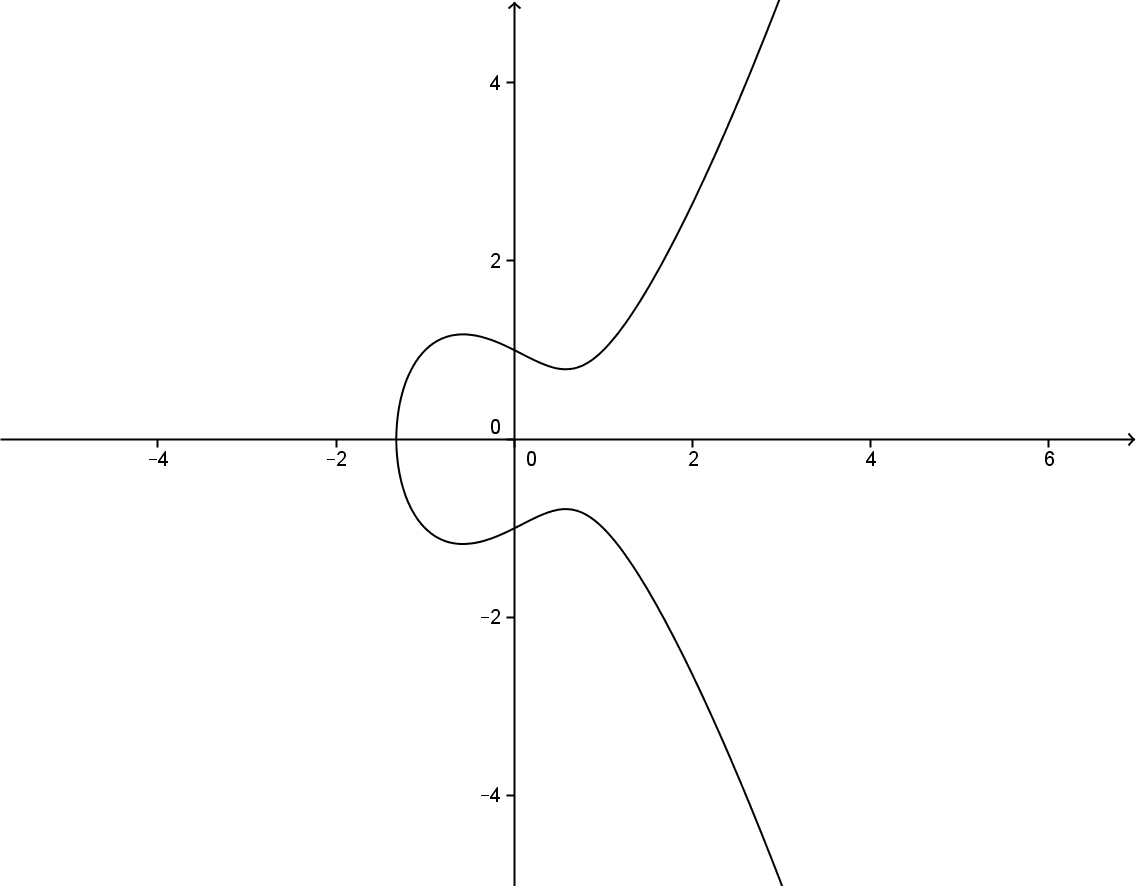
\includegraphics[scale=0.2]{elliptic_1}
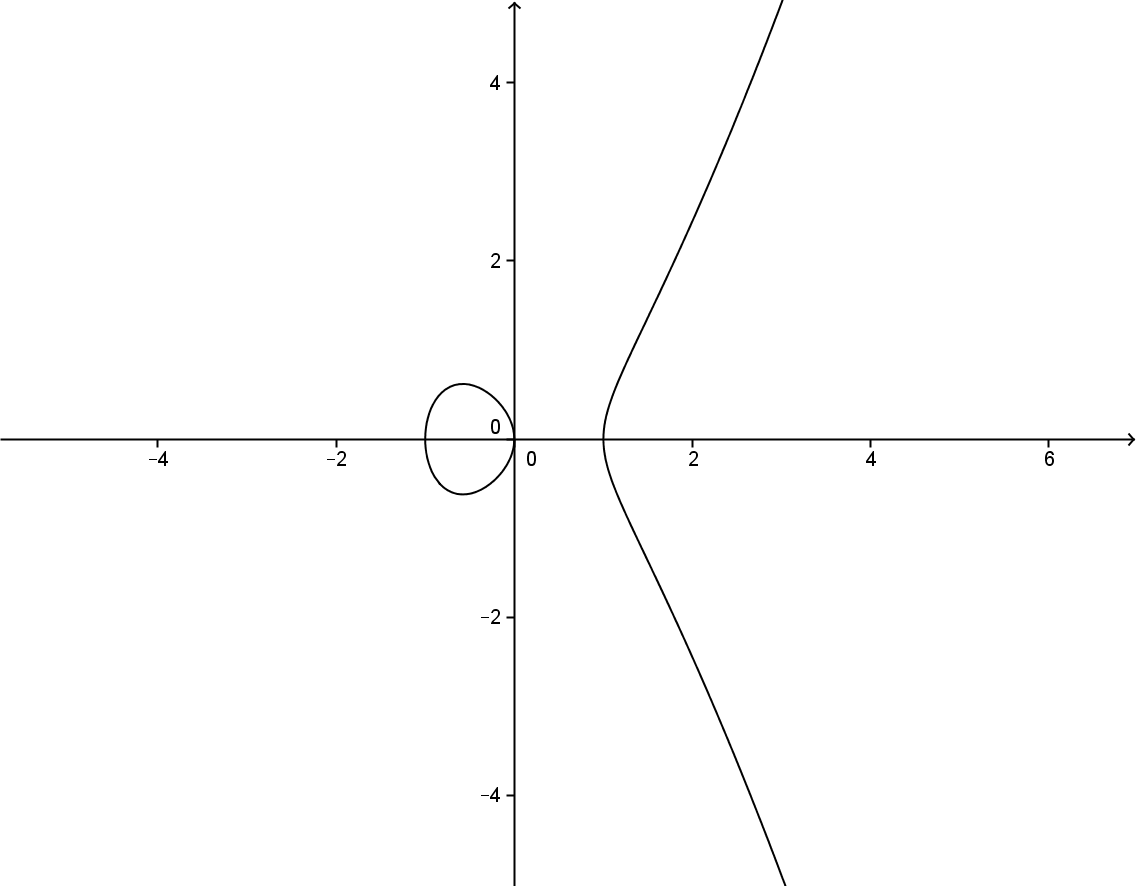
\includegraphics[scale=0.2]{elliptic_2}
\caption{Eksempler på elliptiske kurver over $\mathbb{R}$. Venstre: $y^2 = x^3 - x$, Højre: $y^2 = x^3 -x + 1$}
\end{figure}
Definitionen siger, at $A$ og $B$ skal tilhøre et legeme $K$. Det kunne f.eks. være $\mathbb{R}, \mathbb{C}$ eller $\mathbb{Q}$. Vi vil dog dog fokusere på de endelige legemer $\mathbb{F}_p = \mathbb{Z}/p\mathbb{Z}$ hvor $p$ er et primtal, og de endelige legemer med $q$ elementer $\mathbb{F}_q$, hvor $q = p^r$ for $r \geq 1$ (se appendiks \ref{appendiks_legemer}). Hvis $A, B \in K$ for en elliptisk kurve $E$ siger vi, at $E$ er givet over $K$. Fremover menes en elliptisk kurve på Weierstrass normalform, når vi snakker om en elliptisk kurve $E$. 
Punkterne på en elliptisk kurve med koordinater i et legeme $L \supseteq K$ skriver vi som $E(L)$, hvor 
\begin{align}
\label{elliptic_curve_points}
	E(L) = \{ \infty \} \cup \{ (x, y) \in L \times L \mid y^2 = x^3 + Ax + B \}.
\end{align}
Punktet $\infty$ kaldes punktet i uendelig og viser sig nødvendigt for at $E(L)$ bliver en gruppe under additionen vi introducerer i næste afsnit. Intuitivt kan vi se $\infty$ som værende punktet $(\infty, \infty)$, som er placeret i toppen af $y$-aksen. En linje siges at gå igennem $\infty$ præcist når den er lodret, hvilket betyder at to lodrette linjer skærer hinanden i $\infty$. $\infty$ kan også tænkes som værende i bunden af $y$-aksen, men så vil to lodrette linjer skære hinanden to steder, hvilket er hvorfor vi kræver at punktet $\infty$ i toppen og i bunden er et og samme punkt.

\section{Den projektive plan}
Vi vil i dette afsnit formalisere punktet $\infty$, som vi kort diskuterede ovenfor. For atk unne gøre dette får vi brug for den projektive plan 
$\mathbb{P}^2$. Rent intuitivt kan man se den projektive plan, som
værende den affine plan 
\begin{align*}
	\mathbb{A}^2(K) = \{ (x, y) \in K \times K \},
\end{align*}
hvor $K$ et et legeme, med en ekstra linje "i uendelig". 
Vi ønsker at formalisere dette begreb. 
For $x, y, z \in K$ ikke alle nul og $\lambda \in K$, $\lambda \neq 0$, 
definerer vi en ækvivalensrelation. To tripler $(x_1, y_1, z_1)$ og 
$(x_2, y_2, z_2)$ siges at være ækvivalente hvis 
\begin{align*}
	(x_1, y_1, z_1) = (\lambda x_2, \lambda y_2, \lambda z_2),
\end{align*}
og vi skriver $(x_1, y_1, z_1) \sim (x_2, y_2, z_2)$. Vi vil fremover skrive
$(x:y:z)$ for en sådan ækvivalensklasse. Den projektive plan er da givet ved
\begin{align*}
	\mathbb{P}^2(K) = \{ (x, y, z) \in K^3 \mid (x, y, z) \neq (0, 0, 0)\}/\sim.
\end{align*}
I de tilfælde hvor $z \neq 0$ har vi, at
\begin{align*}
	(x : y : z) = (x/z : y/z : 1),
\end{align*}
hvilket er de punkter vi kalder for de endelige punkter i $\mathbb{P}^2(K)$.
Vi er nemlig i stand til at associere et punkt fra $\mathbb{A}^2(K)$ med et sådan
punkt. Vi har en inklusion $\mathbb{A}^2(K) \hookrightarrow \mathbb{P}^2(K)$ givet ved
\begin{align*}
	(x, y) \mapsto (x : y : 1).
\end{align*}
Dette kan vi selvfølgelig ikke gøre, når $z=0$ og når dette er tilfældet ser vi det som, at enten $x$ eller $y$-koordinaten er $\infty$. Vi kalder dermed punkterne
$(x, y, 0)$ for punkterne i uendelig og punktet $\infty$ på en elliptisk kurve vil vi identificere med netop ét af disse.

Et polynomium siges at være homogent af grad $n$, hvis det er summen af led på formen $ax^i y^j z^k$, hvor $a \in K$ og $i + j + k = n$. Eksempelvis er 
\begin{align*}
	F(x, y, z) = 5x^4 - 2x^2 yz + 7yz^3
\end{align*}
et homogent polynomium af grad $4$. For et homogent polynomium $F$ af grad $n$ er
\begin{align*}
	F(\lambda x, \lambda y, \lambda z) = \lambda^n F(x, y, z), \quad \lambda \in K.
\end{align*}
Vi har altså, at når $(x_1, y_1, z_1) \sim (x_2, y_2, z_2)$ er $F(x_1, y_1, z_1) = 0$ hvis og kun hvis $F(x_2, y_2, z_2) = 0$. Et nulpunkt for $F$ i $\mathbb{P}^{2}(K)$ er altså ikke afhængig af repræsentanten for en given ækvivalensklasse, hvilket betyder at nulpunkterne for $F$ er veldefineret i $\mathbb{P}^{2}(K)$.

For et arbitrært polynomium $F(x, y, z)$ giver det ikke mening, at snakke om et punkt i $\mathbb{P}^2(K)$ hvor $F(x, y, z) = 0$, da det nemlig afhænger af repræsentanten $(x, y, z)$ for ækvivalensklassen. Vi har f.eks., at for
$F(x, y, z) = 2x^2 - y - z$ at $F(1, 1, 1) = 0$, men $F(2, 2, 2) = 4$. Men da $(1 : 1 : 1) = (2 : 2 : 2)$ har vi et problem, som vi undgår ved at arbejde med homogene polynomier i stedet. For et polynomium $f(x, y)$ kan vi homogenisere det ved, at indsætte de korrekte potenser af $z$. F.eks. for $f(x, y) = y^2 - x^3 - Ax - B$ har vi, at $F(x, y) = y^2 z - x^3 - Axz^2 - Bz^3$. Generelt for et polynomium $f(x, y)$ har vi at, hvis
\begin{align*}
	f(x, y) = \sum_{i} a_i x^{p_i} y^{q_i},
\end{align*}
hvor $\max \{p_i + q_i \} = n$, er dets homogene form
\begin{align*}
	F(x, y, z) = \sum_i a_i x^{p_i} y^{q_i} z^{n-p_i - q_i}.
\end{align*}
Dermed har vi, at 
\begin{align*}
	F(x, y, z) &= z^n \sum_i a_i x^{p_i} z^{-p_i} y^{q_i} z^{-q_i} = z^n \sum_i a_i \left( \frac{x}{z} \right)^{p_i}
	\left( \frac{y}{z} \right)^{q_i} \\  
	&= z^n f\left( \frac{x}{z}, \frac{y}{z} \right).
\end{align*}
Da er det klart, at 
\begin{align*}
	f(x, y) = F(x, y, 1).
\end{align*}
Vi er nu i stand til at undersøge, hvad det vil sige for to parallelle linjer at mødes i uendelig. Lad først
\begin{align*}
	y = mx + b_1, \quad y = mx + b_2,
\end{align*}
være to linjer, som ikke er lodrette og hvor $b_1 \neq b_2$. Homogeniserer vi dem, som forklaret ovenfor, får vi
\begin{align*}
	y = mx + b_1z, \quad y = mx + b_2 z.
\end{align*}
Trækker vi ligningerne fra hinanden får vi, at 
\begin{align*}
	0 = (b_1 - b_2)z \Rightarrow z = 0,
\end{align*}
hvilket så betyder, at $y = mx$. Da vi ikke kan have, at både $x, y$ og $z$ er $0$ samtidigt må vi have $x \neq 0$. Vi kan da dele med $x$ og vi får, at skæringen er
\begin{align*}
	(x : mx : 0) = (1 : m : 0).
\end{align*}
Dette er et af punkterne i uendelig fra $\mathbb{P}^2(K)$.
På samme måde har vi, at hvis $x=c_1$ og $x=c_2$ er lodrette linjer, at de skærer hinanden i punktet $(0 : 1 : 0)$. Dette er også ét af de punkter, som vi identificerede som værende et punkt i uendelig i $\mathbb{P}^2(K)$.

Hvis vi nu homogeniserer ligningen for en elliptisk kurve $E$ med variablen $z$ får vi, at
\begin{align*}
\label{homogeniseret_weierstrass}
	y^2 z = x^3 + Ax z^2 + B z^3.
\end{align*} 
For at se hvilke punkter i uendelig, som er på $E$ sætter vi $z=0$. Dette giver os, at $0 = x^3$ hvilket har en tredobbelt rod i $x=0$ og $y$ kan være et hvilket som helst tal som ikke er $0$, da vi ikke kan have $(0 : 0 : 0)$. 
Efter en skalering med $y$ har vi $(0 : y : 0) = (0 : 1 : 0)$ så $(0 : 1 : 0)$ er det eneste punkt i uendelig på $E$. Da $(0 : 1 : 0)$ er et punkt på enhver lodret linje skærer enhver lodret linje $E$ i dette punkt i uendelig. Vi har desuden, da $(0 : 1 : 0) = (0 : -1 : 0)$, at punkterne i uendelig i toppen og bunden af $y$-aksen er de samme.

Vi vil dog her foretrække, at arbejde med affine koordinater, hvor punktet $\infty$ behandles som et specialtilfælde, men vi har nu givet konkret mening til punktet $\infty$.

\section{Gruppeloven}
Lad $E$ være en elliptisk kurve over et legeme $K$. Det viser sig, at vi kan tage to punkter (eller blot ét) på $E$ og producere et tredje punkt som også er på $E$. Vi vil i dette afsnit vise, hvordan dette gøres og til slut konkludere, at defineres dette som en additions operator bliver $E(K)$ en additiv abelsk gruppe. Vælg to punkter
\begin{align*}
	P_1 = (x_1, y_1) \quad \text{og} \quad P_2 = (x_2, y_2)
\end{align*}
på $E$. 
\begin{figure}
\label{figure_addition_law}
\centering
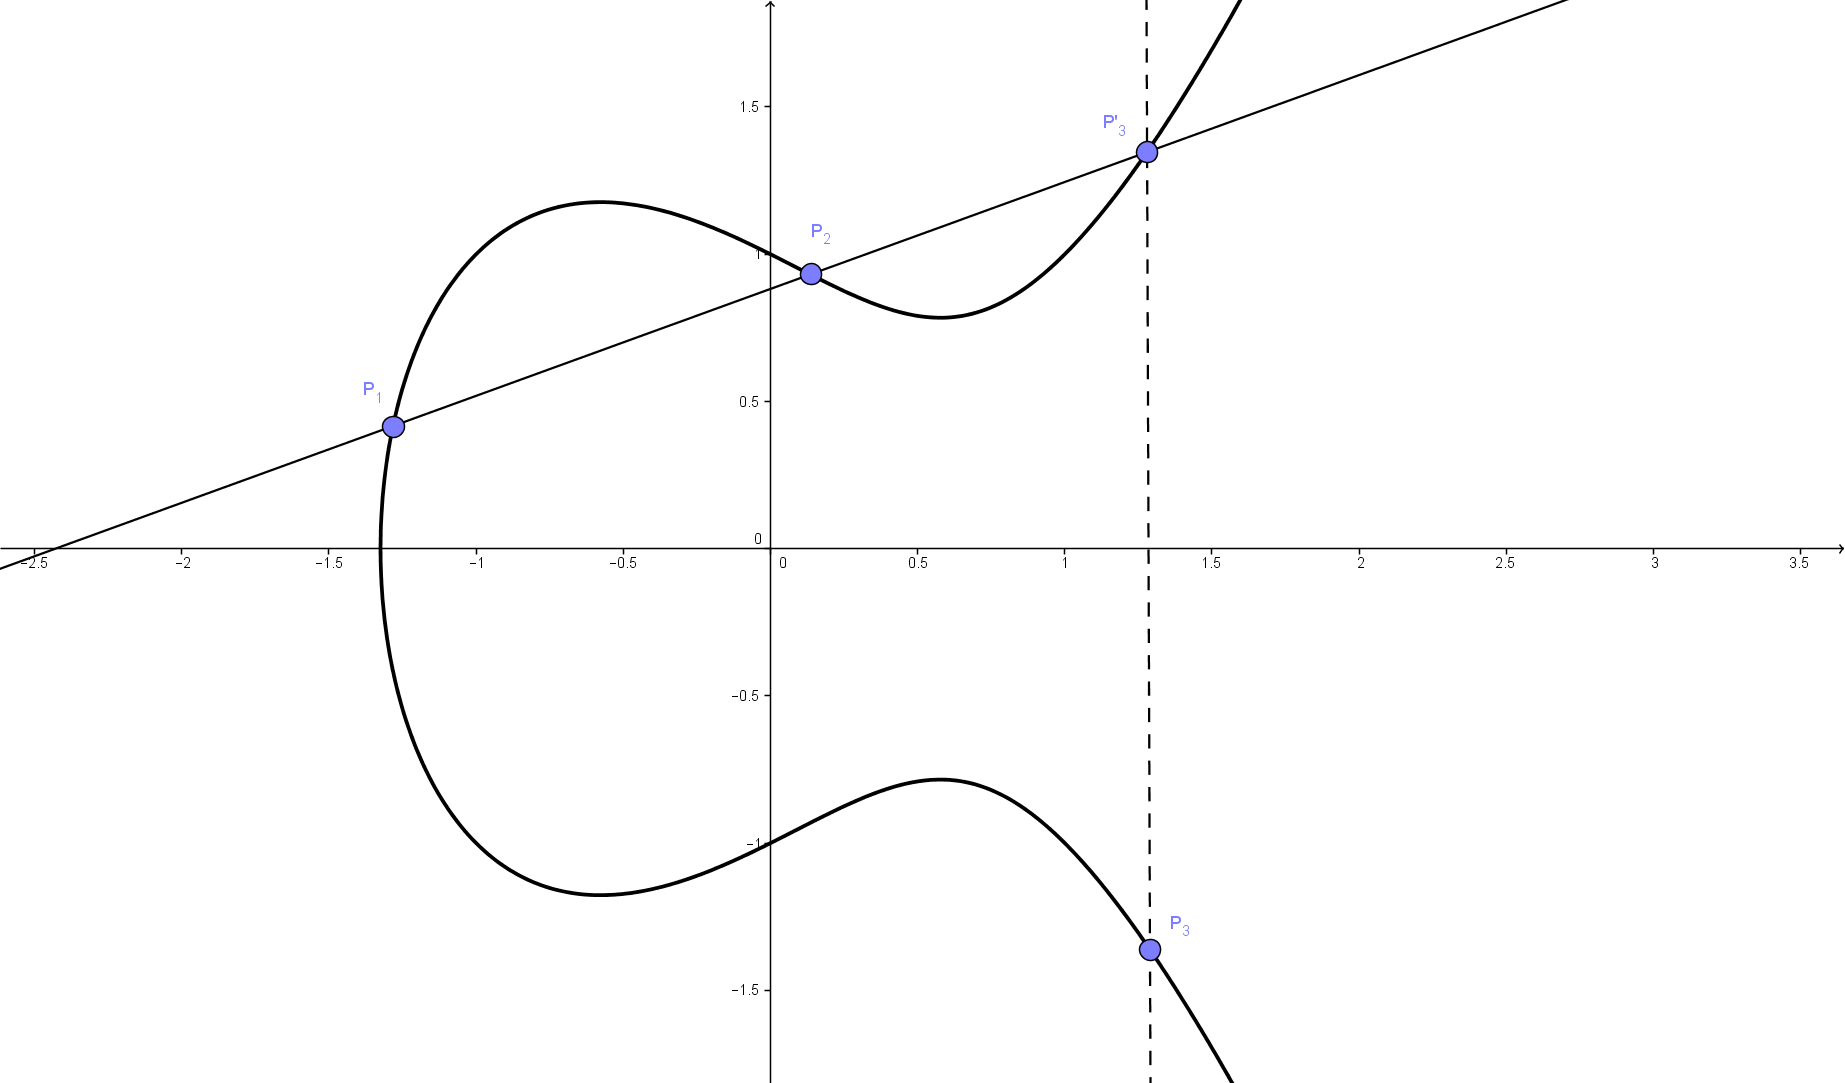
\includegraphics[scale=0.25]{elliptic_1_better}
\caption{Addition af to punkter på en elliptisk kurve}
\end{figure}
Vi kan da trække en ret linje $L$ igennem punkterne $P_1$ og $P_2$, som så vil skære kurven for $E$ i et tredje punkt ${P_3}'$ (se appendiks for bevis om skæring i 3 punkter). Vi definerer $P_1 + P_2 = P_3$ til at være reflektionen i $x$-aksen af dette punkt. 

Vi vil nu udlede formlerne for denne addition af punkter på $E$. Antag først, at $P_1 \neq P_2$ og lad $P_1$ og $P_2$ være forskellige fra $\infty$. Vi har da, at hældningen for linjen der går igennem $P_1$ og $P_2$ er
\begin{align*}
	m = \frac{y_2 - y_1}{x_2 - x_1}.
\end{align*}
Hvis $x_1 = x_2$ er linjen lodret, hvilket er et tilfælde som vi behandler senere. Antag altså at $x_1 \neq x_2$, vi har da
\begin{align*}
	y_2 = m(x_2 - x_1) + y_1.
\end{align*}
Vi indsætter dette i ligningen for $E$ og får, at 
\begin{align*}
	(m(x-x_1) + y_1)^2 = x^3 + Ax + B.
\end{align*}
Skrives dette ud får vi, at
\begin{align*}
	0 &= x^3 + Ax + B - 2y_1 m(x-x_1) - m^2 (x - x_1)^2 - y_{1}^{2} \\
	&= x^3 + Ax + B - 2y_1 m x - 2y_1 m x_1 - m^2 (x^2 -2x x_1 + x_{1}^{2}) - y_{1}^{2} \\
	&= x^3 - m^2 x^2 + (A-2my_1 +2m^2x_1)x -2m y_1 x_1 -m^2 x_{1}^{2} - y_{1}^{2} + B. 
\end{align*}
Denne har tre rødder, som netop er de tre punkter, hvor $L$ skærer $E$.
Pr. vores konstruktion kender vi allerede de to rødder $x_1$ og $x_2$,
og vi ønsker at finde den tredje. Generelt for et kubisk polynomium 
$x^3 + ax^2 + bx + c$, med rødder $r, s, t$, har vi at 
\begin{align*}
	x^3 + ax^2 + bx + c = (x - r)(x - s)(x - t) = x^3 - (r + s + t)x^2 + \ldots,
\end{align*}
hvilket giver os, at $-a = r + s + t$. Hvis de to rødder vi kender er $r$ og $s$
kan vi finde den sidste som
\begin{align*}
	t = -a - r - s.
\end{align*}
I vores tilfælde er $a=-m^2$ så vi har, at 
\begin{align*}
	x = m^2 - x_1 - x_2.
\end{align*}
Vi mangler da blot at reflektere dette punkt for at have fundet 
punktet $P_1 + P_2 = P_3 = (x, y)$. Vi reflekterer over $x$-aksen og finder, at 
\begin{align*}
	x = m^2 - x_1 - x_2, \quad y = m(x_1 - x) - y_1.
\end{align*}
Vi vender nu tilbage til tilfældet, hvor $x_1 = x_2$. Da vil linjen igennem 
$P_1$ og $P_2$ være lodret, så den skærer $E$ i $\infty$. Vi husker, at når $\infty$ 
reflekteres over $x$-aksen får vi igen $\infty$. Vi får altså, at $P_1 + P_2=\infty$.

Tilfældet hvor $P_1 = P_2 = (x_1, y_1)$ kræver lidt flere overvejelser. For to punkter som ligger
tæt på hinanden vil linjen igennem punkterne nærme sig tangenten til et af punkterne. Når vi har to ens punkter lader vi da linjen igennem dem være tangenten til punktet. Ved implicit differentiation finder vi, at 
\begin{align*}
	2y \frac{dy}{dx} = 3x^2 + A, \quad \text{så} \quad m = \frac{dy}{dx} = \frac{3x_{1}^{2} + A}{2y_1}.
\end{align*}
Hvis $y_1 = 0$ er linjen lodret og i det tilfælde lader vi $P_1 + P_2 = \infty$. Antag altså, at $y_1 \neq 0$. Ligningen for $L$ er 
\begin{align*}
	y = m(x-x_1) + y_1,
\end{align*}
som før. Vi får den kubiske ligning
\begin{align*}
	0 = x^3 - m^2 x^2 + \ldots
\end{align*}
Vi kender dog kun én rod, $x_1$, men den er en dobbelt rod idet at $L$ er tangent til $E$ i $P_1$. Så på samme måde som før får vi, at 
\begin{align*}
	x_3 = m^2 - 2x_1, \quad y_3 = m(x_1 - x_3) - y_1.
\end{align*}
Antag nu, at $P_2 = \infty$. Linjen som går igennem $P_1$ og $\infty$ er en lodret linje, som skærer $E$ i reflektionen af $P_1$ over $x$-aksen. Når vi reflekterer dette punkt igen over $x$-aksen får vi igen $P_1$. Altså har vi, at
\begin{align*}
	P_1 + \infty = P_1.
\end{align*}
Denne definition udvides sådan, at $\infty + \infty = \infty$.

Det er nu mere klart, hvorfor elliptiske kurver og denne definition for en addition passer sammen. Højresiden i en ligning på Weierstrass normalform er kubisk så en linje igennem to punkter skærer den i et tredje punkt. At venstresiden er $y^2$ sikrer os, at kurven er symmetrisk om $x$-aksen, som benyttes når vi reflekterer et punkt. Vi opsummerer denne diskussion og kan opstille gruppeloven:

\begin{definition}[Gruppeloven]
\label{gruppeloven:definitionen}
Lad $E$ være en elliptisk kurve. Givet to punkter, $P_1, P_2 \in E(K)$, $P_i = (x_i, y_i)$, findes et tredje punkt $P_3 = P_1 + P_2 = (x_3, y_3)$ da som følger
\begin{enumerate}
	\item Hvis $x_1 \neq x_2$ er 
	\begin{align*}
		x_3 = m^2 - x_1 - x_2, \quad y_3 = m(x_1 - x_3) - y_1,
	\end{align*}		
	hvor $m = (y_2 - y_1)/(x_2 - x_1)$.
	\item Hvis $x_1 = x_2$, men $y_1 \neq y_2$ da er $P_1 + P_2 = \infty$.
	\item Hvis $P_1 = P_2$ og $y_1 \neq 0$ er 
	\begin{align*}
		x_3 = m^2 - 2x_1, \quad y_3=m(x_1 - x_3) - y_1,
	\end{align*}
	hvor $m=(3{x_1}^2 + A)/2y_1$.
	\item Hvis $P_1 = P_2$ og $y_1 = 0$ da er $P_1 + P_2 = \infty$.
\end{enumerate}
Vi definerer desuden, at 
\begin{align*}
	P + \infty = \infty,
\end{align*}
for alle $P \in E(K)$.
\end{definition}
Det måske overraskende hovedresultatet i dette kapitel er, at denne addition resulterer i en abelsk gruppe:

\begin{thm}
Punkterne på $E$, altså $E(K)$, udgør en additiv abelsk gruppe hvor $\infty$ er identiteten og additionen er som defineret i gruppeloven. 
\end{thm}
\begin{proof}
For at være en gruppe skal additionen af punkter være kommutativ, der skal eksistere en identitet, hvert element skal have en invers og additionen af punkter skal være associativ.

Kommutativiteten kan enten ses direkte fra formlerne eller fra det faktum, at linjen igennem $P_1$ og $P_2$ er den samme som linjen igennem $P_2$ og $P_1$. At $\infty$ er identiteten følger pr. definitionen af denne. For de inverse elementer lader vi $P'$ være reflektionen af $P$, da er $P+P' = \infty$. Associativiteten kan vises direkte ud fra formlerne, men der er mange tilfælde der skal behandles, hvilket gør det besværligt. Et bevis for associativiteten kan findes i \cite[afsnit~2.4]{Washington} eller i \cite{Silverman}.
\end{proof}